\subsection{Sample Collection}

\subsubsection{Wastewater Sampling Points}
The performance study of wastewater treatment is done using experimental data obtained from the laboratory at the \ac{WWTP} in Moratuwa/Ratmalana. The quality of inlet and outlet wastewater was tested on a daily and weekly basis in the laboratory. pH, temperature, \ac{TDS}, \ac{DO}, and color at inlet and outlet wastewater, as well as \ac{SV30} and \ac{DO} levels of the aerobic tank, were tested daily as operational parameters. Also, pH, temperature, \ac{TDS}, \ac{TSS}, \ac{OG} concentration, fluoride, \ce{NO3-} (As N), \ce{PO4-} (As P), \ac{DO}, color at the inlet and outlet wastewater, and \ac{MLSS}, \ac{MLVSS}, \ac{F/M Ratio}, \ac{TS}, \ac{DO}, \ac{SV30}, and \ac{SVI} in the aerobic tank were tested weekly as verification parameters.

This performance evaluation has been conducted through the process of comparison. The data collection process involved gathering information over a period of 30 weeks from both the inlet and outlet of the treatment plant. The collected data parameters were inlet flow, pH, temperature, \ac{BOD5}, \ac{COD}, \ac{TSS}, fluoride, \ce{PO4-} (As P), and \ac{OG}. Each week included one data set for each parameter of the inlet and outlet, and during this evaluation, each sample was renamed with a unique sample number, as mentioned in \cref{table:sample_numbering}.  In the last 5 weeks of the data collection period, I actively worked with the lab assistant to test the parameters. All the tests related to the collected data have been done according to the procedures outlined in the Standard Methods for the Examination of Water and Wastewater \cite{APHA}.


\begin{figure}[H]
\centering
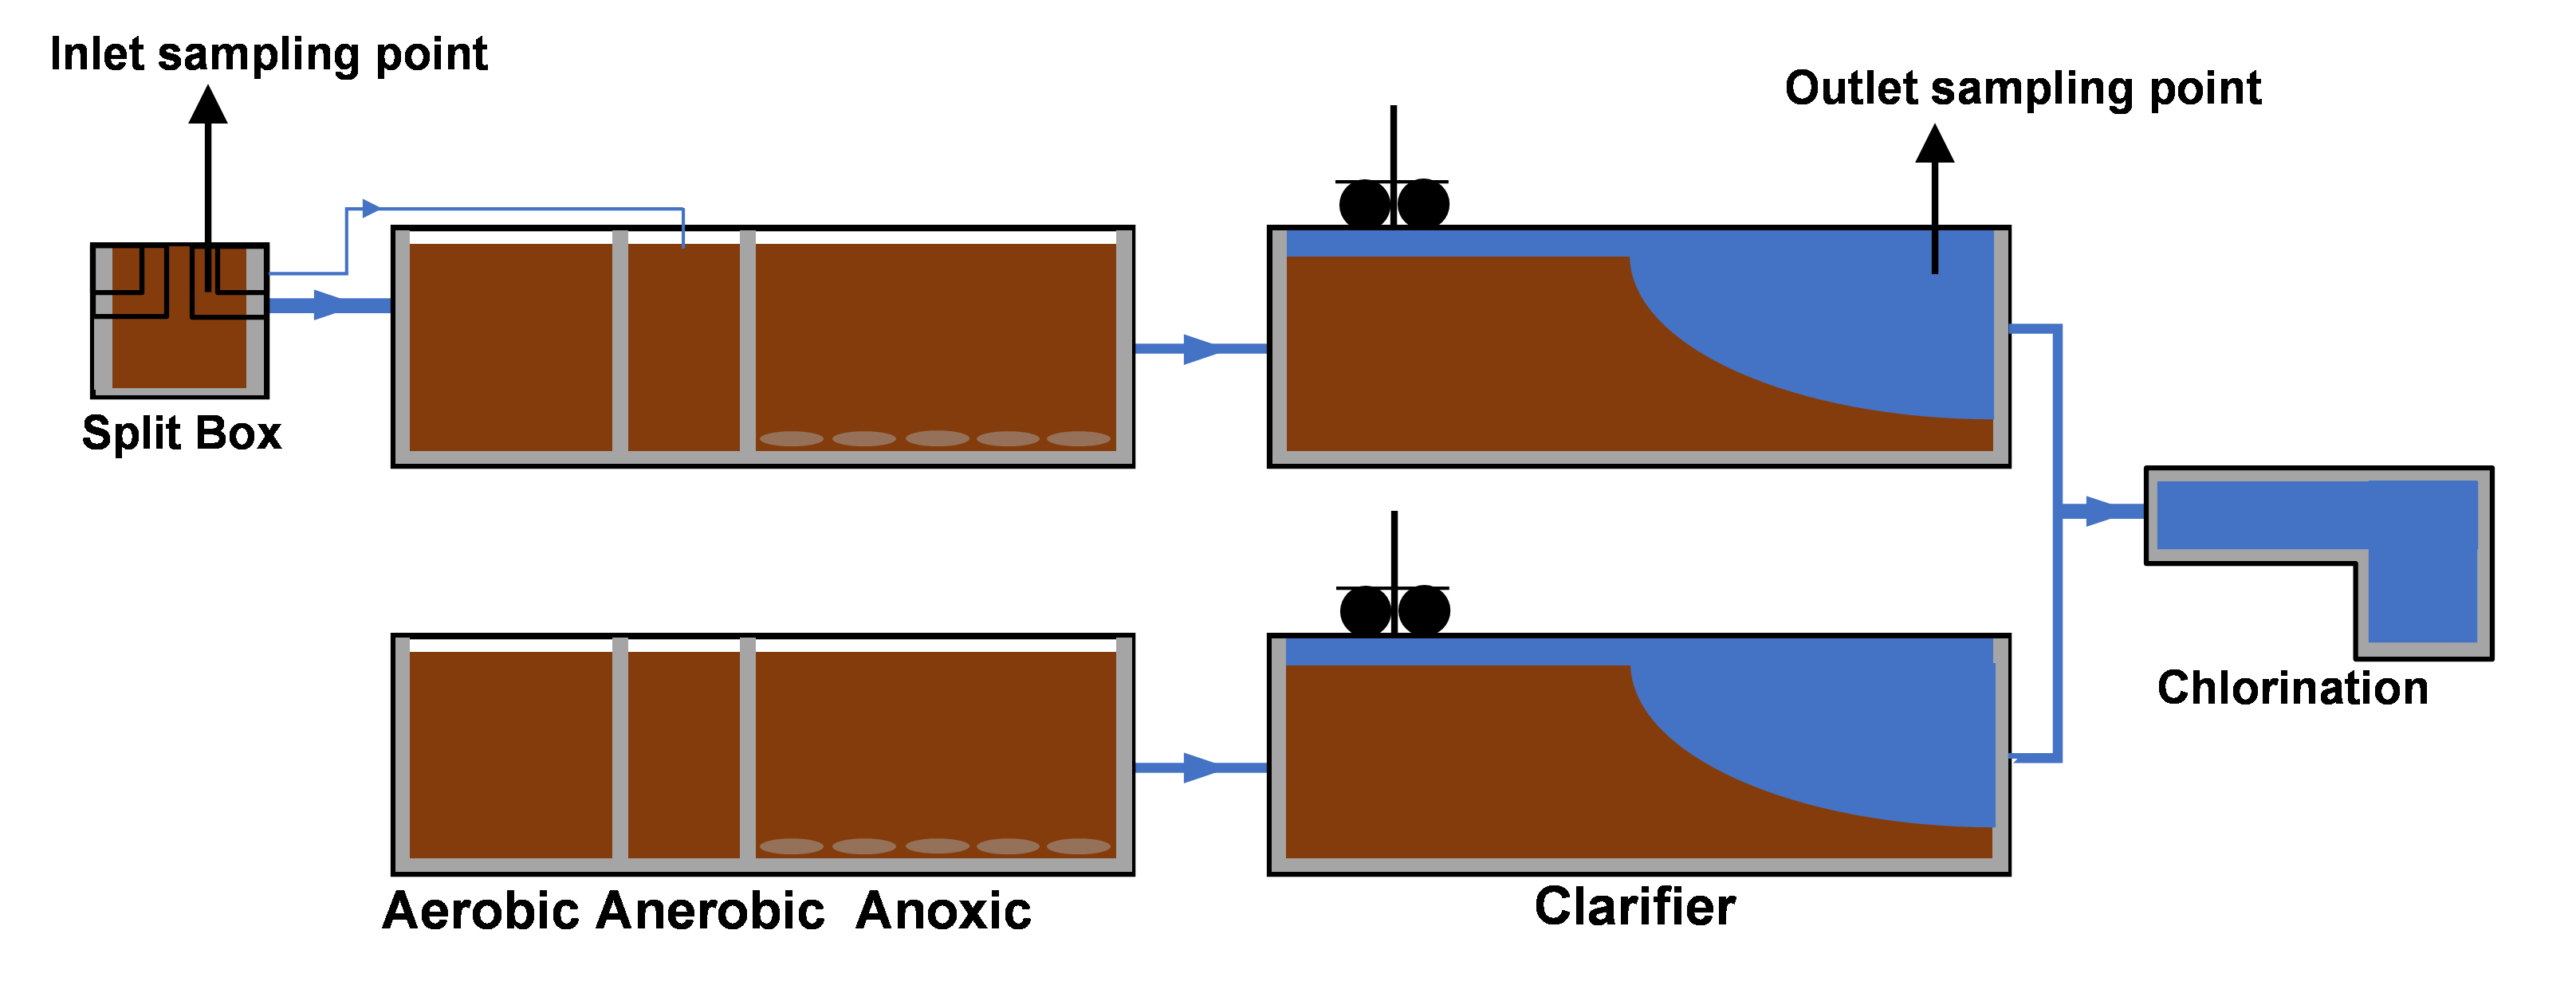
\includegraphics[width=1\linewidth]{material_and_methodology/sample_point_inlet_outlet.png}


\caption{Inlet and outlet sampling points}
\label{fig:sample_points_inlet_outlet}
\end{figure}



\subsubsection{Sludge Sampling Points}
The samples were collected from three locations, and the analyzed parameters and number of samples from December to February are shown below:

\begin{table}[H]
\caption{Sample details related to the sludge}
\centering
\begin{tabular}{|>{\centering\arraybackslash}p{1.5cm}|l|l|>{\centering\arraybackslash}p{2cm}|l|}
\hline
Sample Name & Sample Location & Sample Description & Number of Samples & Tested Parameters \\
\hline
$S_1$ & Sludge storage tank & Thickened sludge & 1 & TSS \\
\hline
$S_2$ & Dewatered unit & Reject water & 1 & TSS \\
\hline
$S_3$ & Dewatered unit & Dewatered sludge & 3 & Moisture content \\
\hline
$S_4$  & Sludge drying bed & Dried sludge & 15 & Moisture content \\
\hline
\end{tabular}

\label{table:sample_details}
\end{table}

Three $S_4$ samples mentioned in \cref{table:sample_details} were collected from three sampling points in a line, as shown in \cref{fig:samples_collected_points}, to analyze the moisture content of dried sludge, and 10 mg of each sample was mixed and one sample named as $S_5$ was prepared. The remaining four samples ($S_5$) were prepared  in the same manner using other $S_4$ samples.

\begin{figure}[H]
\centering
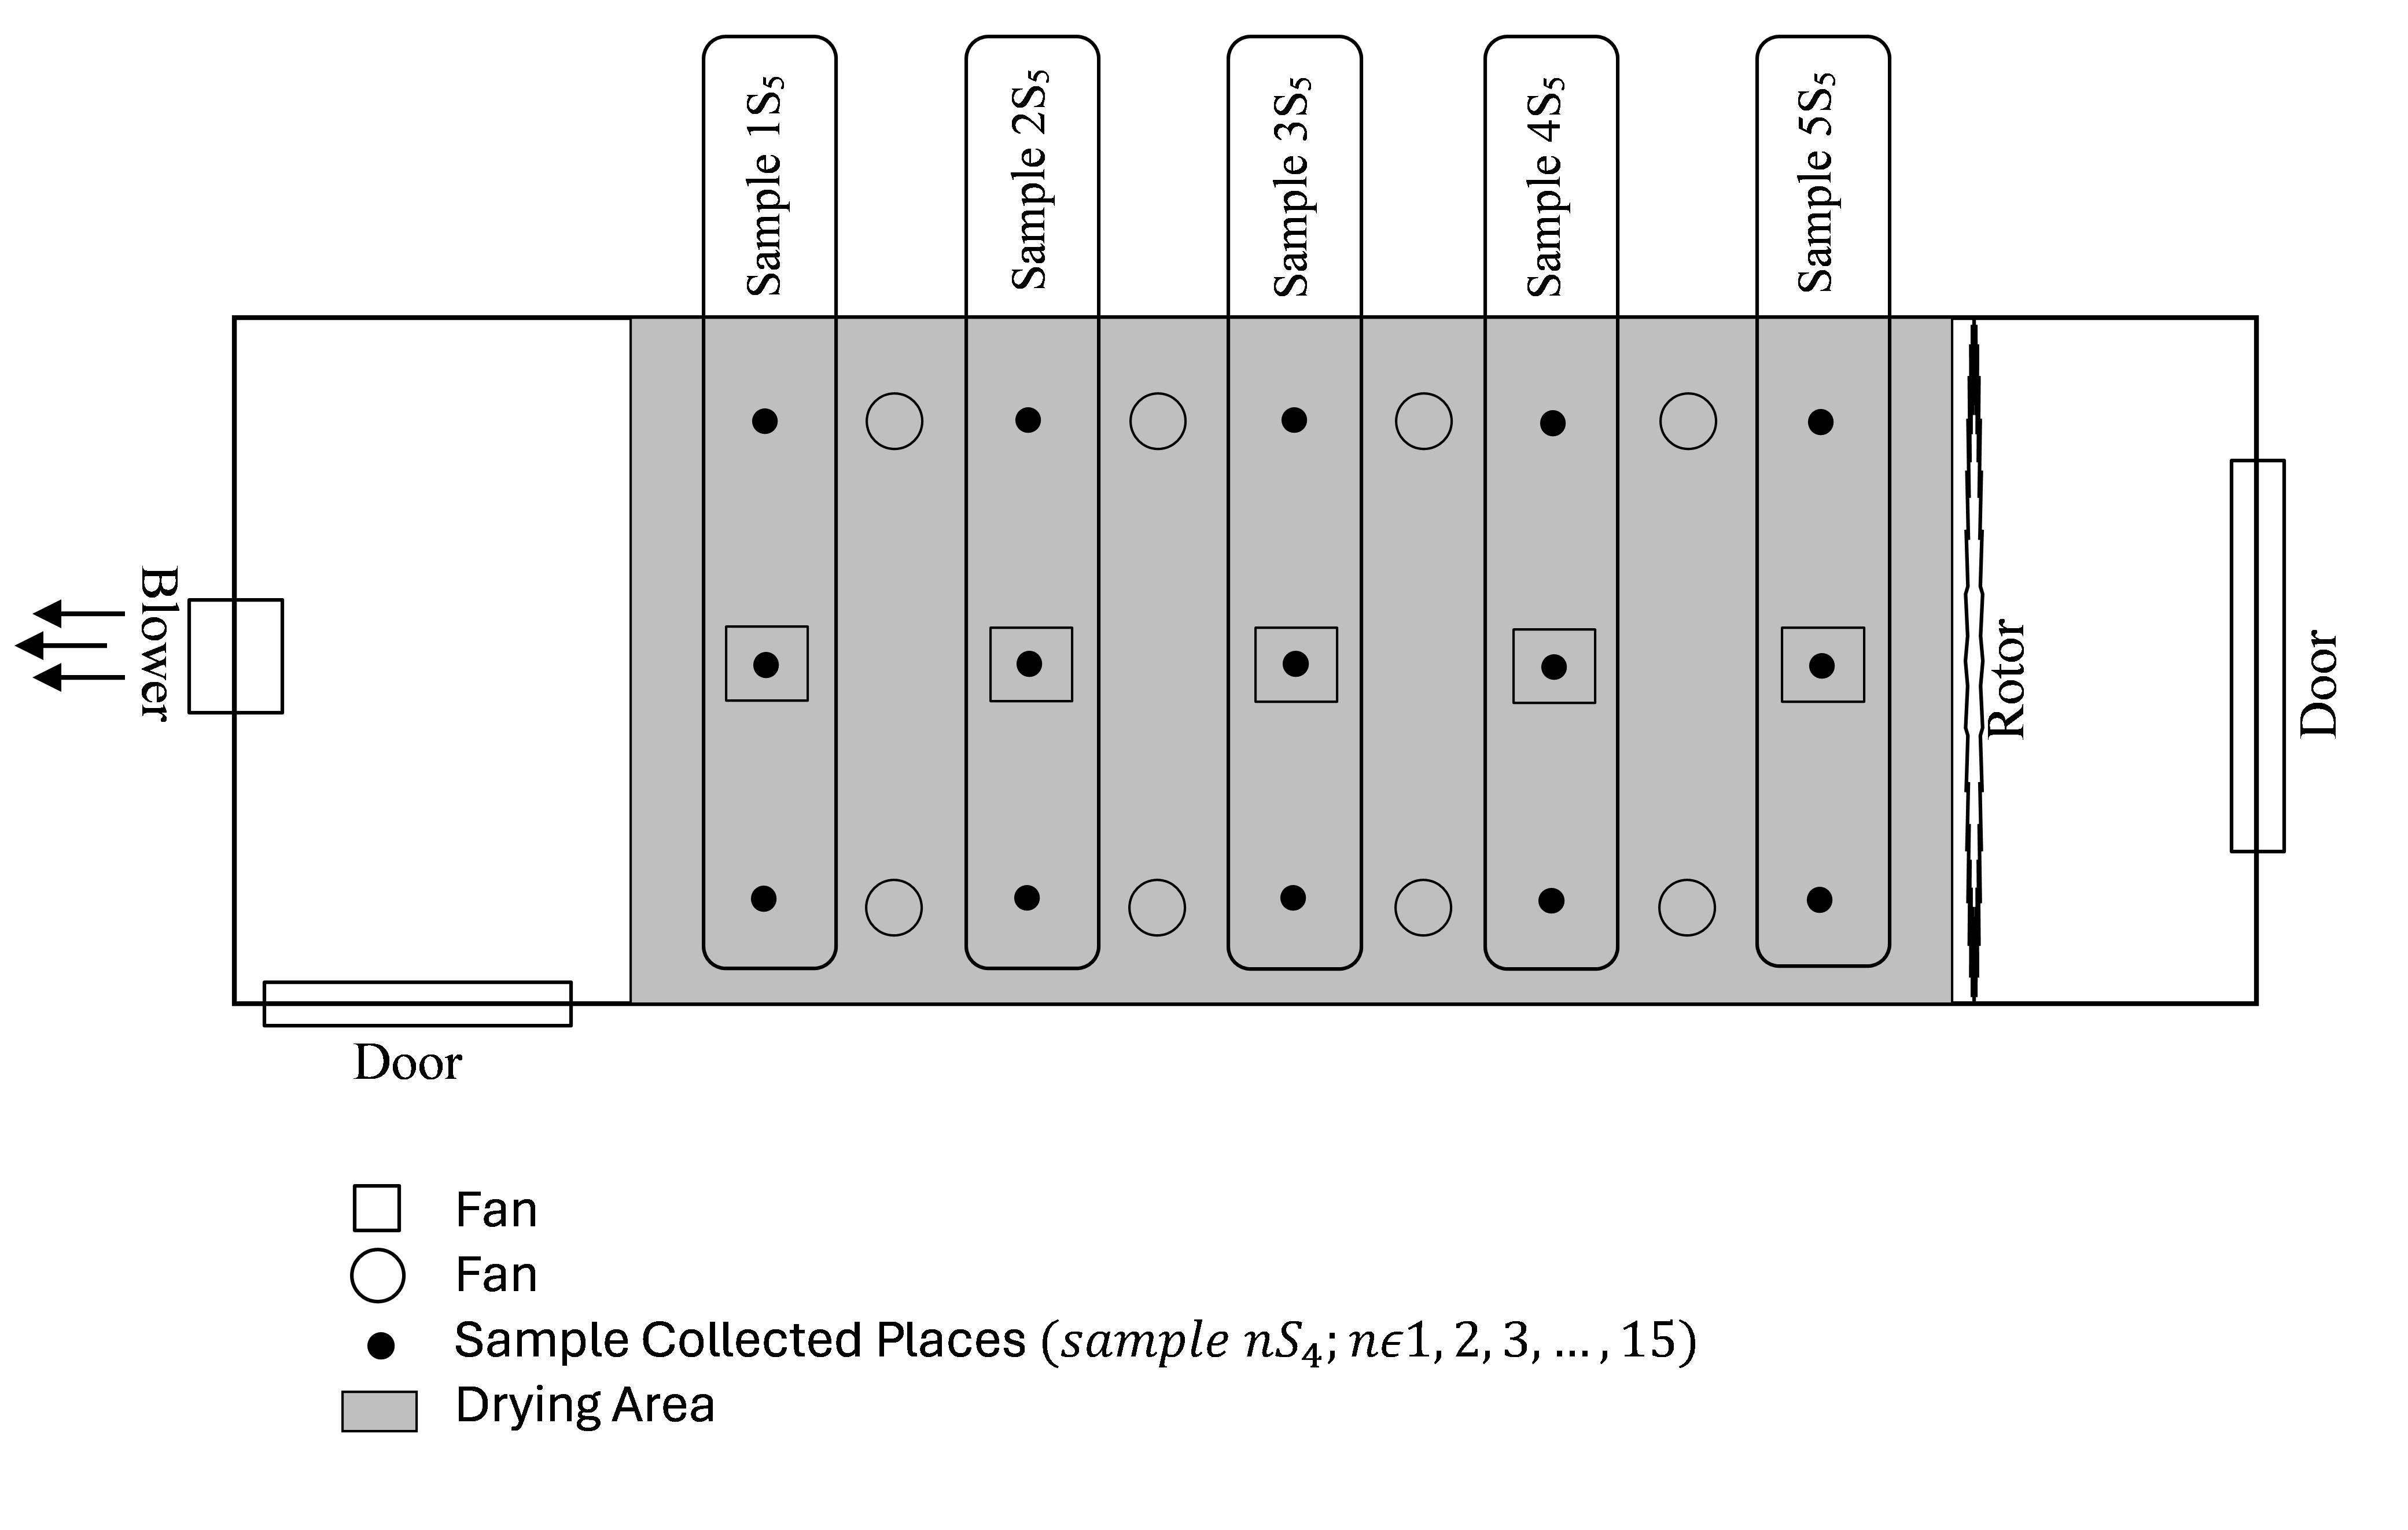
\includegraphics[width=1\linewidth]{material_and_methodology/sample_collected_point_dryingbed.png}
\caption{Samples collected points in the drying bed}
\label{fig:samples_collected_points}
\end{figure}


\subsection{Determination of Total Suspended Solid}
Two dry and clean glass microfiber filter papers with watch glasses were weighed, and sample $S_1$ and sample $S_2$ mentioned in \cref{table:sample_details} were filtered using pre-weighed glass microfiber filter papers. Each piece of filtered paper was kept on the watch glass and stored at 105 ℃ for 1 hour. After 1 hour, samples were removed and placed in a desiccator until they reached a constant weight. Then, samples were weighted, and \ac{TSS} was calculated using the below formula:

\begin{equation}
    \text{TSS} = \dfrac{\text{Weight of suspended solid (\unit{mg})}}{\text{Volume of water filtered (\unit{l})}}
\end{equation}

\subsection{Determination of Moisture Content}
Dry and clean aluminum foil containers were weighted, and used to tare the balance. Three samples of $S_3$ mentioned in \cref{table:sample_details} and five samples of $S_5$  were added to each container and measured for weight. Then, the samples were stored at 105 °C for 18 hours. After 18 hours, samples were removed and placed in a desiccator until they reached a constant weight. Then, samples were weighted, and moisture content was calculated using the below formula:

\begin{equation}
    \text{Moisture Content} = \dfrac{\text{Wet weight of sludge (\unit{g})} - \text{Dry weight of sludge (\unit{g})}}{\text{Wet weight of sludge (\unit{g})}} \times 100\%
\end{equation}

\subsection{Determination of Removal Efficiency}
The removal efficiency of the various parameters was estimated using the below formula:

\begin{equation}
    \text{Removal Efficiency} = \dfrac{\text{influent} \left( \unit{mg/l} \right) - \text{effluent} \left( \unit{mg/l} \right) }{\text{influent} \left( \unit{mg/l} \right)}
\end{equation}

\subsection{Correlation}
The data was collected over a period of one year (from January to December 2023) to identify the correlation between the \ac{TSS} and \ac{BOD5} parameters. Initially, data collection included 53 datasets related to the \ac{TSS} and \ac{BOD5} of the inlet. First of all, outliers were removed from the data set using Excel software, and the remaining 50 data points were used for the process. The first 30 data points were selected for the statistical regression tests, considering \ac{TSS} as the independent variable and \ac{BOD5} as the dependent variable, and then the remaining 20 samples were used to compare the laboratory results with the regression test results. The statistical analysis was conducted using the R language and Excel software.\cite{Kumar2010, Nikoonahad2016}.

 